\documentclass{ctexart}
\usepackage{geometry}
\usepackage[dvipsnames,svgnames]{xcolor}
\usepackage{framed}
\usepackage{enumerate}
\usepackage{amsmath,amsthm,amssymb}
\usepackage{enumitem}
\usepackage{template}
\usepackage{tikz}

\usetikzlibrary{patterns}
\allowdisplaybreaks
\geometry{left=2cm, right=2cm, top=2.5cm, bottom=2.5cm}

\begin{document}
\pagestyle{empty}
\begin{center}\large Cauchy-Schwarz不等式\end{center}
一个理想的释经学者应该是一位去过第一世纪那个奇异世界的人,感觉到其中的一片陌生,
但却在那里逗留,知道自己生活在其中,他的思想和感受与初听福音的人一样为止;
然后再回到今日的世界,将所获悉的真理用我们今日的思想诉说出来.\hfill—— Charles Harold Dodd\\\ \\
让我们从实数域上离散形式的Cauchy不等式开始.
\begin{formal}[1.1]
    已知$a_1,\cdots,a_n,b_1,\cdots,b_n$均为实数,则有
    $$\left(\sum_{i=1}^{n}a_ib_i\right)^2\leqslant\left(\sum_{i=1}^{n}a_i^2\right)\left(\sum_{i=1}^{n}b_i^2\right)$$
\end{formal}
\begin{solution}[Proof.]
    置$\displaystyle A_i=\dfrac{a_i}{\sqrt{\sum_{i=1}^{n}a_i^2}},B_i=\dfrac{b_i}{\sqrt{\sum_{i=1}^{n}b_i^2}}$,
    则根据基本不等式有$$A_iB_i\leqslant\dfrac{A_i^2+B_i^2}{2}$$
    即$$\dfrac{a_ib_i}{\sqrt{\sum_{i=1}^{n}a_i^2}\sqrt{\sum_{i=1}^{n}b_i^2}}\leqslant\dfrac{1}{2}\left(\dfrac{a_i^2}{\sum_{i=1}^{n}a_i^2}+\dfrac{b_i^2}{\sum_{i=1}^{n}b_i^2}\right)$$
    对不等式两边求和有$$\dfrac{\sum_{i=1}^{n}a_ib_i}{\sqrt{\sum_{i=1}^{n}a_i^2}\sqrt{\sum_{i=1}^{n}b_i^2}}\leqslant\dfrac{1}{2}\left(\dfrac{\sum_{i=1}^{n}a_i^2}{\sum_{i=1}^{n}a_i^2}+\dfrac{\sum_{i=1}^{n}b_i^2}{\sum_{i=1}^{n}b_i^2}\right)=1$$
    移项后两边平方即可得$$\left(\sum_{i=1}^{n}a_ib_i\right)^2\leqslant\left(\sum_{i=1}^{n}a_i\right)\left(\sum_{i=1}^{n}b_i\right)$$
    原命题得证.
\end{solution}\noindent
基本不等式$ab\leqslant\dfrac{a^2+b^2}{2}$具有一个直观的几何解释.
我们注意到在下面的图中,长方形的面积为$ab$,两个三角形的面积分别为$\dfrac{1}{2}a^2,\dfrac{1}{2}a^2$.
显然,长方形的面积不大于两个三角形面积之和,误差项为阴影处的小三角形的面积.
于是就有$$ab\leqslant\dfrac{a^2+b^2}{2},\text{等号成立当且仅当}a=b$$
\begin{center}
    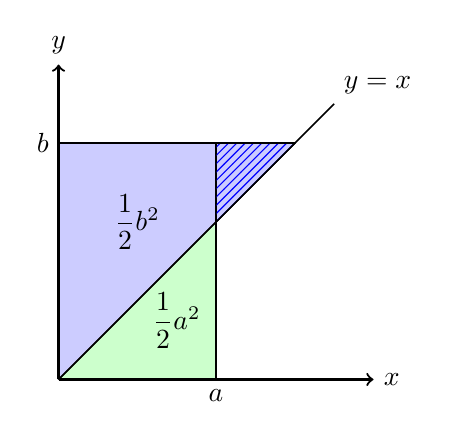
\begin{tikzpicture}
        \filldraw[fill=blue!20] (0,0)--(3,3)--(0,3)--(0,0);
        \filldraw[fill=green!20] (0,0)--(2,2)--(2,0)--(0,0);
        \draw[line width=0.8pt,->] (0,0)--(4,0) node[right]{$x$};
        \draw[line width=0.8pt,->] (0,0)--(0,4) node[above]{$y$};
        \draw[line width=0.6pt] (0,0)--(3.5,3.5);
        \node[above right] at(3.5,3.5) {$y=x$};
        \draw[line width=0.6pt] (2,0)--(2,3);
        \draw[line width=0.6pt] (0,3)--(3,3);
        \node[below] at(2,0) {$a$};
        \node[left] at(0,3) {$b$};
        \node at(1.5,0.75) {$\dfrac{1}{2}a^2$};
        \node at(1,2) {$\dfrac{1}{2}b^2$};
        \filldraw[pattern color=blue,pattern=north east lines] (2,2)--(3,3)--(2,3)--(2,2);
    \end{tikzpicture}
\end{center}
我们可以根据这个图形写出如下式子.
$$ab\leqslant\dfrac{a^2+b^2}{2}=\int_0^ax\dx+\int_0^by\di y$$
能否对这个式子做推广呢?事实上,我们有
\begin{formal}[1.2 Young's不等式]
    函数$y=\phi(x)\in C([0,+\infty))$且在定义域上严格单调递增,满足$\displaystyle\phi(0)=0,\lim_{x\to+\infty}\phi(x)=+\infty$.则
    $$ab\leqslant\int_0^ay\dx+\int_0^bx\di y\ \ \forall a,b>0$$
\end{formal}
\begin{solution}[Proof.]
    若$b>\phi(a)$,则有
    $$\begin{aligned}
        \int_0^ay\dx+\int_0^b x\di y
        &= \int_0^ay\dx+\int_0^{\phi(a)}x\di y+\int_{\phi(a)}^{b}x\di y\\
        &= \int_0^ay\dx+\int_0^{a}xy'\dx+\int_{\phi(a)}^{b}(x-a)\di y+\int_{\phi(a)}^{b}a\di y\\
        &= \int_0^a(y+xy')\dx+\int_{\phi(a)}^{b}(x-a)\di y+a(b-\phi(a))\\
        &= \left.xy\right|_0^a+ab-a\phi(a)+\int_{\phi(a)}^{b}(x-a)\di y \\
        &= ab+\int_{\phi(a)}^{b}(x-a)\di y \\
    \end{aligned}$$
    由$y=\phi(x)$严格递增可知$\forall y>\phi(a),x>a$,于是$\displaystyle\int_{\phi(a)}^b(x-a)\di y>0$.
    于是就有$$\int_0^ay\dx+\int_0^b x\di y>ab$$
    若$b=\phi(a)$,容易验证不等式取等.\\
    若$b<\phi(a)$,同理可以得到
    $$\int_0^ay\dx+\int_0^b x\di y=ab+\int_{\phi^{-1}(b)}^a(y-b)\dx>ab$$
    从而题设不等式成立.
\end{solution}\noindent
我们在Young's不等式中令$y=\phi(x)=x^{p-1},p>1$,则$\phi^{-1}(y)=y^{\frac{1}{p-1}}$.于是
$$ab\leqslant\dfrac{a^p}{p}+\dfrac{b^{1+\frac{1}{p-1}}}{1+\frac{1}{p-1}}\ \ \forall a,b\geqslant 0$$
置$q=1+\dfrac{1}{p-1}$,则$\dfrac{1}{p}+\dfrac{1}{q}=\dfrac{1}{p}+\dfrac{p}{p-1}=1$,上述式子可以改写为
\begin{theorem}[1.2.Special Form]
    对于任意$p,q>1$满足$\dfrac{1}{p}+\dfrac{1}{q}=1$,有
    $$ab\leqslant\dfrac{a^p}{p}+\dfrac{b^q}{q}\ \ \forall a,b\geqslant0$$
\end{theorem}\noindent
应用上面的引理,我们马上可以证明Hölder's不等式.
\begin{formal}[1.3.1 Hölder's不等式 I]
    设$a_1,\cdots,a_n,b_1,\cdots,b_n$均为非负实数,$p,q>1$且$\dfrac{1}{p}+\dfrac{1}{q}=1$,则有
    $$\sum_{i=1}^{n}a_ib_i\leqslant\left(\sum_{i=1}^{n}a_i^p\right)^{\frac{1}{p}}\left(\sum_{i=1}^{n}b_i^q\right)^{\frac{1}{q}}$$
\end{formal}\noindent
特别的,当$p=q=2$时上式记为Cauchy-Schwarz不等式.我们采用相似的方法证明之.
\begin{solution}[Proof.]
    置$A_i=\dfrac{a_i}{\left(\sum_{i=1}^{n}a_i^p\right)^{\frac{1}{p}}},B_i=\dfrac{b_i}{\left(\sum_{i=1}^{n}b_i^q\right)^{\frac{1}{q}}}$,于是根据Young's不等式有
    $$A_iB_i\leqslant\dfrac{A_i^p}{p}+\dfrac{B_i^q}{q}=\dfrac{a_i^p}{p\sum_{i=1}^{n}a_i^p}+\dfrac{b_i^q}{q\sum_{i=1}^{n}b_i^q}$$
    对不等式两边求和有$$\dfrac{\sum_{i=1}^na_ib_i}{\left(\sum_{i=1}^na_i^p\right)^{\frac{1}{p}}\left(\sum_{i=1}^nb_i^q\right)^{\frac{1}{q}}}\leqslant\dfrac{\sum_{i=1}^{n}a_i^p}{p\sum_{i=1}^{n}a_i^p}+\dfrac{\sum_{i=1}^{n}b_i^q}{q\sum_{i=1}^{n}b_i^q}=\dfrac{1}{p}+\dfrac{1}{q}=1$$
    移项即可得$$\sum_{i=1}^{n}a_ib_i\leqslant\left(\sum_{i=1}^{n}a_i^p\right)^{\frac{1}{p}}\left(\sum_{i=1}^{n}b_i^q\right)^{\frac{1}{q}}$$
    原命题得证.
\end{solution}\noindent
同样的,Hölder's不等式也有积分形式.
\begin{formal}[1.3.2 Hölder's不等式 II]
    已知$f(x),g(x)\in C([a,b]),p,q>1\text{且}\dfrac{1}{p}+\dfrac{1}{q}=1$,则有
    $$\left|\int_a^bf(x)g(x)\dx\right|\leqslant\left(\int_a^b\left|f(x)\right|^p\dx\right)^{\frac{1}{p}}\left(\int_a^b\left|g(x)\right|^q\dx\right)^{\frac{1}{q}}$$
\end{formal}
\begin{solution}[Proof.]
    设$T:\left\{x_i\right\}_{i=0}^n$为$[a,b]$上的一个分割,满足$a=x_0<x_1<\cdots<x_{n-1}<x_n=b$.\\
    记$\displaystyle\Delta x_i=x_i-x_{i-1},\lambda=\max_{1\leqslant i\leqslant n}\left\{\Delta x_i\right\}$,于是根据Riemann积分的定义有
    $$\begin{aligned}
        \left|\int_a^bf(x)g(x)\dx\right| &= \lim_{\lambda\to0^+}\sum_{i=1}^{n}\left|f(x_i)\right|\left|g(x_i)\right|\Delta x_i \\
        \int_a^b\left|f(x)\right|^p\dx &= \lim_{\lambda\to0^+}\sum_{i=1}^n\left|f(x_i)\right|^p\Delta x_i \\
        \int_a^b\left|g(x)\right|^q\dx &= \lim_{\lambda\to0^+}\sum_{i=1}^n\left|g(x_i)\right|^q\Delta x_i
    \end{aligned}$$    
    根据1.3.1的结论,我们有
    $$\sum_{i=1}^{n}\left|f(x_i)\right|\left|g(x_i)\right|\leqslant\left(\sum_{i=1}^{n}\left|f(x_i)\right|^p\right)^{\frac{1}{p}}\left(\sum_{i=1}^{n}\left|g(x_i)\right|^q\right)^{\frac{1}{q}}$$
    控制$\Delta x_i$相同,则有
    $$\lim_{\lambda\to0^+}\sum_{i=1}^{n}\left|f(x_i)\right|\left|g(x_i)\right|\Delta x_i\leqslant\left(\lim_{\lambda\to0^+}\sum_{i=1}^n\left|f(x_i)\right|^p\Delta x_i\right)^{\frac{1}{p}}\cdot\left(\lim_{\lambda\to0^+}\sum_{i=1}^n\left|g(x_i)\right|^q\Delta x_i\right)^{\frac{1}{q}}$$
    于是就有
    $$\left|\int_a^bf(x)g(x)\dx\right|\leqslant\left(\int_a^b\left|f(x)\right|^p\dx\right)^{\frac{1}{p}}\left(\int_a^b\left|g(x)\right|^q\dx\right)^{\frac{1}{q}}$$
    从而题设不等式成立.
\end{solution}
\end{document}